% =====================================================================
%  HotMobile 2027 — COMBINED position paper (CPU + Apple Silicon).
%  Drafted 2026-08-06. Separate from main.tex (the Paper-1-only port).
%  Deadline: 9 Oct 2026 11:59pm AoE · <=6pp · sigconf 10pt · non-anonymous
%  Build:  tectonic combined.tex     (or: latexmk -pdf combined.tex)
%  TODO before submission:
%    (1) Figure 1 — combined prefill-fraction curve for both platforms,
%        generated from the two released datasets. Placeholder below.
%    (2) Swap in HotMobile's official 10pt-amended acmart template if provided.
%    (3) Add CCS concepts (required for camera-ready, optional at submission).
% =====================================================================
\documentclass[sigconf,nonacm,10pt]{acmart}

\usepackage{booktabs}
\usepackage{graphicx}
% acmart already provides amsmath, amssymb, hyperref, natbib, xcolor

\settopmatter{printacmref=false}
\renewcommand\footnotetextcopyrightpermission[1]{}
\pagestyle{plain}
\setcopyright{none}
\emergencystretch=2em

\begin{document}

\title{The Bottleneck Moves Twice: Three Regimes of
On-Device LLM Latency}

\author{Bapista Khan}
\affiliation{%
  \institution{Collab-Foundry}
  \country{}}
\email{bapistakhan@gmail.com}
\renewcommand{\shortauthors}{Bapista Khan}

\begin{abstract}
On-device language models are increasingly deployed for privacy, offline operation and cost, yet the latency
intuition the community carries is inherited from datacentre GPU serving, where autoregressive \emph{decode}
dominates. We instrumented end-to-end inference across two on-device platforms and four model sizes, and found
that the bottleneck does not merely differ between devices---\textbf{it moves, twice, on a single device, as a
function of context length alone}. On an 8\,GB Apple Silicon device a 3B model is \emph{decode-bound} at short
context (prefill 20\% of latency), becomes \emph{prefill-bound} through the middle (peaking at 80\% near 1{,}500
tokens), and then \emph{re-inverts} toward decode past $\sim$2{,}029 tokens as weights plus KV cache exhaust
unified memory and decode throughput collapses from 49 to 17\,tok/s. Smaller models on the same device never
reach the third regime; a CPU-only machine, by contrast, never leaves the second, climbing monotonically to
95\% prefill. \textbf{How many regimes a deployment traverses is set by the headroom between model footprint
and memory capacity}---which makes it a design-time property, not a runtime detail. We argue this has immediate
consequences for how the mobile systems community benchmarks, schedules and budgets on-device inference, and
that single-number throughput reporting conceals all three transitions. Harnesses and raw data are released.
\end{abstract}

\keywords{on-device inference, mobile systems, LLM, latency, prefill, memory wall, measurement}

\maketitle

% =====================================================================
\section{Introduction}

Running language models on the device rather than in the datacentre is no longer exotic. Privacy requirements,
offline operation, and the cost of inference at scale have pushed capable models onto phones, laptops and edge
hardware~\cite{xu2024ondevicereview,liu2024mobilellm,xue2024powerinfer2}. The engineering intuition that
travelled with them did not come from those devices. It came from GPU serving, where the dominant cost is
autoregressive \emph{decode} and where optimisation effort---batching, paged attention, speculative
decoding---has been directed accordingly~\cite{kwon2023pagedattention,leviathan2023speculative}.

We took that intuition to two on-device platforms and measured it. It does not merely fail. It fails
\emph{differently at different context lengths on the same machine}.

On an 8\,GB Apple Silicon device, a 3B model is \textbf{decode-bound} at short context---prefill accounts for
only 20\% of end-to-end latency. As context grows it becomes \textbf{prefill-bound}, peaking at 80\% near
1{,}500 tokens. Then, past roughly 2{,}029 tokens, it \textbf{re-inverts}: prefill's share falls back to
$\sim$69\% while decode throughput collapses from 49 to 17\,tok/s, as weights plus a growing KV cache exhaust
unified memory. Nothing changed but the length of the prompt.

Smaller models on the same device never reach that third regime---0.5B and 1.5B climb monotonically and their
decode throughput declines only gently, because their footprint leaves headroom. A CPU-only machine sits at the
other extreme: across the whole sweep it never leaves the prefill-bound regime, climbing monotonically from 38\%
to \textbf{95\%}.

So the number of regimes a deployment traverses is not a property of the platform alone. It is set by the
\textbf{headroom between model footprint and memory capacity}---which makes it something a developer chooses at
design time, usually without knowing they are choosing it.

\paragraph{Contributions.}
\begin{itemize}
  \item We identify \textbf{three distinct latency regimes} for on-device inference and show a single device
        traversing all three as context grows (\S\ref{sec:three}).
  \item We show which regimes a configuration reaches is governed by memory headroom, not platform class
        (\S\ref{sec:three}), and give the mechanism for both transitions (\S\ref{sec:why}).
  \item We draw out what follows for benchmarking, scheduling and context budgeting, and argue that
        single-number throughput reporting conceals every transition (\S\ref{sec:implications}).
  \item We release both harnesses and all raw data (\S\ref{sec:repro}).
\end{itemize}

\section{Three Regimes}
\label{sec:three}

\paragraph{Setup.} Both studies sweep prompt length from 55 to 2{,}336 tokens with five repetitions per point,
discard warm-up runs, and instrument prefill and decode separately end to end. Platform~A is a CPU-only machine
(AMD Ryzen~7 8845HS, 8 cores / 16 threads, 14\,GiB) running quantized Qwen2.5-7B, Llama-3.1-8B and Gemma2-9B
through \texttt{llama.cpp}~\cite{gerganov2023llamacpp}. Platform~B is an 8\,GB MacBook Air running 4-bit MLX
builds of Qwen2.5-Instruct at 0.5B, 1.5B and 3B---a deliberate size sweep on a device where larger families do
not comfortably fit, which turns out to be the point. Every number traces to a released raw-results file.

\begin{table}[t]
\caption{The three regimes. The binding constraint changes, and with it the only lever that helps.}
\label{tab:regimes}
\small
\begin{tabular}{@{}llll@{}}
\toprule
\textbf{Regime} & \textbf{Signature} & \textbf{Bound by} & \textbf{Lever} \\
\midrule
1. Decode-bound  & prefill $<$50\%              & sequential cost & output length \\
2. Prefill-bound & prefill rising, $>$50\%      & compute         & context length \\
3. Memory-bound  & prefill \emph{falling},      & capacity        & KV growth \\
                 & decode collapsing            &                 &            \\
\bottomrule
\end{tabular}
\end{table}

\begin{table}[t]
\caption{One device, three regimes. Qwen2.5-3B (4-bit) on an 8\,GB Apple Silicon machine: prefill share rises,
peaks, then \emph{reverses} as decode collapses past the memory wall. Means over five repetitions.}
\label{tab:traversal}
\small
\begin{tabular}{@{}rrrl@{}}
\toprule
\textbf{Context} & \textbf{Prefill} & \textbf{Decode} & \textbf{Regime} \\
(tokens)         & (\% of latency)  & (tok/s)         &                 \\
\midrule
   55 & 19.9 & 49.5 & 1 · decode-bound \\
  140 & 35.4 & 49.2 & 1 \\
  300 & 50.5 & 49.2 & $\rightarrow$ 2 · crossover \\
  600 & 64.6 & 49.2 & 2 · prefill-bound \\
 1000 & 74.5 & 48.4 & 2 \\
 1500 & \textbf{79.9} & 43.5 & 2 · peak \\
 2000 & 68.8 & \textbf{23.5} & $\rightarrow$ 3 · memory wall \\
 2336 & 69.4 & \textbf{17.3} & 3 · memory-bound \\
\bottomrule
\end{tabular}
\end{table}

\begin{figure}[t]
  \centering
  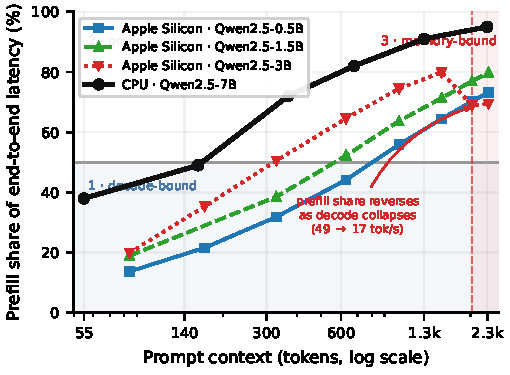
\includegraphics[width=\columnwidth]{fig_combined.pdf}
  \caption{Prefill's share of end-to-end latency against context length. The CPU
  (black) climbs monotonically to 95\%: it never leaves regime~2. On Apple Silicon
  the smaller models climb and level off, while \textbf{Qwen2.5-3B peaks near
  1{,}500 tokens and then reverses}---not because prefill became cheap, but because
  decode collapsed past the memory wall. Means over five repetitions; one flagged
  1.5B outlier excluded.}
  \label{fig:combined}
\end{figure}

Table~\ref{tab:traversal} is the paper. A developer who profiles this configuration at 600 tokens and one who
profiles it at 2{,}300 tokens will reach opposite conclusions about what to optimise, on identical hardware
running an identical model.

\paragraph{Headroom decides how far you travel.} On the same device, Qwen2.5-0.5B climbs monotonically from
13.7\% to 73.2\% prefill with decode declining only gently (250 to 208\,tok/s), and 1.5B behaves the same way
(19.0\% to 79.9\%; 96 to 87\,tok/s).\footnote{One anomalous 1.5B point near 140 tokens is excluded, as in the
underlying study.} Neither reaches regime~3, because neither exhausts unified memory. Only the 3B model---the
one whose weights plus KV cache approach the 8\,GB ceiling---re-inverts.

\paragraph{Some platforms never leave regime 2.} Platform~A shows no reversal anywhere in the sweep. Prefill
climbs monotonically---38\% at 55 tokens, 72\% at 367, 91\% at 1{,}299, \textbf{95\%} at 2{,}336---while decode
sits flat at 11--12\,tok/s. With 14\,GiB and a 7B model there is ample headroom, so memory never binds; the
machine simply lacks the parallelism to make prefill cheap. Llama-3.1-8B and Gemma2-9B reproduce this at
95--96\% prefill, and the effect reproduces on a second CPU vendor (Intel Comet Lake), where it is if anything
stronger.

\paragraph{The crossover between regimes~1 and~2 also moves with model size,} and in the direction that
surprises people: \emph{earlier} for larger models---$\sim$1{,}029 tokens at 0.5B against $\sim$329 at 3B.
Bigger models reach the prefill-bound regime sooner and the memory-bound regime sooner.

\paragraph{Quantization does not behave as the folklore says.} On Platform~A prefill \emph{speed} is
non-monotonic in footprint: the 8-bit build prefills fastest and an intermediate K-quant slowest, inverting the
``quantize down for speed'' heuristic~\cite{dettmers2022llmint8,frantar2023gptq,lin2024awq}. Smaller is not
reliably faster. What smaller reliably buys is \emph{headroom}---and headroom is what keeps a deployment out of
regime~3.

\section{Why the Bottleneck Moves}
\label{sec:why}

Two transitions, two mechanisms.

\paragraph{Regime 1 $\rightarrow$ 2.} Prefill is a single pass over the context and is parallel across tokens;
it is compute-bound. Decode is sequential---each token depends on the last---and is bound by memory bandwidth,
streaming weights and a growing KV cache at every
step~\cite{kwon2023pagedattention,agrawal2024sarathi}. Prefill cost therefore scales with context while decode
cost per token does not, so prefill eventually overtakes. On hardware that parallelises prefill well this takes
a long prompt; on a CPU it happens almost immediately, which is why Platform~A appears to start in regime~2.
The datacentre disaggregation literature separates the two phases for exactly this
reason~\cite{patel2024splitwise,zhong2024distserve}; on-device there is nowhere to disaggregate to.

\paragraph{Regime 2 $\rightarrow$ 3.} Unified memory holds weights and KV cache in one pool. As context grows
the cache grows with it, and once the combined footprint approaches capacity, decode does not taper---it falls
off a cliff, 49 to 17\,tok/s in our measurements. Because prefill's share is a \emph{ratio}, decode getting
dramatically slower makes prefill look smaller: the curve turns back down. The reversal is not prefill becoming
cheap. It is decode becoming catastrophic. Work on streaming weights from flash addresses a neighbouring
constraint~\cite{alizadeh2024llmflash}, but what we observe is a discontinuity on a device a user is holding.

This is why the three are regimes rather than points on a curve. In regime~1 the lever is output length; in
regime~2 it is context length; in regime~3 neither helps and the only remedy is to reduce footprint. An
optimisation that works in one is neutral or harmful in another.

\section{What This Means for Mobile Systems}
\label{sec:implications}

\paragraph{1. Single-number benchmarks conceal every transition.}
Reporting ``tokens per second'' collapses two phases with opposite scaling into one figure, and says nothing
about which regime produced it. Two devices reporting the same figure can behave completely differently as a
user's context grows. On-device benchmarks should report prefill and decode separately at minimum, and prefill
\emph{fraction against context length} by preference---a curve, not a number. The shape of that curve is the
diagnostic: monotonic means two regimes, rise-then-fall means three.

\paragraph{2. Profiling at one context length is profiling one regime.}
Table~\ref{tab:traversal} makes this concrete: the same configuration profiled at 600 and at 2{,}300 tokens
yields opposite optimisation advice. Any measurement reported without its context length is close to
meaningless.

\paragraph{3. Placement and offload decisions inherit the wrong prior.}
Routing and cascade systems typically cost a request by expected output
length~\cite{chen2023frugalgpt,ong2024routellm,schuster2022calm}. That is right in regime~1, wrong in regime~2,
and dangerously wrong in regime~3, where the true cost is that the request has pushed the device past a cliff
it will not recover from until the context shrinks.

\paragraph{4. The memory wall is a design-time constraint.}
Because it is a discontinuity rather than a slope, on-device capability is not gracefully degradable. An
assistant that behaves well carrying 1{,}800 tokens of history may be unusable at 2{,}200 on the same phone.
That determines how much conversation history a product can keep---an architecture decision, not a tuning flag.
And since headroom is what governs it, choosing a smaller model is often better understood as buying regime
avoidance than as buying speed.

\paragraph{5. Context budgeting is the largest available lever in regime 2.}
If latency is governed by what the model reads, then what it reads is the thing to control. We demonstrated
this on Platform~A: gating the costliest optional stage of an agent pipeline---a second ``review/verify'' model
pass---cut end-to-end latency \textbf{2.4$\times$} with no measurable quality loss under an order-swapped LLM
judge~\cite{zheng2023judging}. It is the largest single lever on that platform, and it is invisible to anyone
optimising decode.

\section{Open Questions}
\label{sec:open}

\paragraph{Can a runtime detect which regime it is in, and adapt?} This is the question we find most
interesting, and the three-regime picture sharpens it into something tractable. The signals are cheap and
already available at inference time---prefill fraction, decode throughput, memory headroom---and each regime has
a known corresponding action: shorten output in regime~1, budget context in regime~2, cap KV growth or swap to
a smaller model in regime~3. A runtime that classified its own regime and switched policy would need no
platform-specific tuning from the developer. Whether such a controller is stable near the boundaries, and
whether the regime-3 transition can be predicted rather than merely detected after the collapse, we do not know.

\paragraph{Is there a fourth regime?} Neither platform includes a dedicated neural accelerator. An NPU may add
one, or may sit inside an existing regime. If regimes keep accumulating, the argument for measuring rather than
assuming strengthens.

\paragraph{Do architectural changes remove a regime or add one?} Mixture-of-experts alters what must be
resident during decode; speculative decoding attacks the sequential dependency that makes decode
slow~\cite{leviathan2023speculative}. Both act directly on the mechanisms above. Whether they collapse regimes
together or separate them further is empirical, and we have not answered it.

\paragraph{Limitations.} Each platform is a single machine, with a second CPU vendor as the only cross-device
check. We measure three model sizes on Platform~B and three families on Platform~A, at one primary quantization
level each. Absolute figures are characteristic of these devices. The claim we defend is the \emph{structure}:
three regimes, two transitions, governed by memory headroom---and that survives across models and across two
CPU vendors.

\section{Conclusion}

On-device LLM latency has no single characterisation, and not merely because devices differ. The bottleneck
moves \emph{within} a device: decode-bound at short context, prefill-bound through the middle, and memory-bound
once weights plus KV cache stop fitting---at which point prefill's share falls not because prefill got cheap but
because decode collapsed. Whether a deployment sees one regime, two or three is decided by the headroom a
developer leaves, usually without realising it is a decision. Any system that schedules, places or budgets
on-device inference---and any benchmark that reports its speed---should measure the hardware and the context
length together, rather than inherit an intuition from a datacentre it will never run in.

\section*{Reproducibility}
\label{sec:repro}
% =====================================================================

Both harnesses, all raw per-run data, and the analysis scripts are public.

\begin{itemize}\itemsep2pt
  \item CPU study\\
        \texttt{\small github.com/bapista/cpu-llm-latency}\\
        DOI 10.5281/zenodo.21765705
  \item Apple Silicon study\\
        \texttt{\small github.com/bapista/mlx-llm-latency}\\
        DOI 10.5281/zenodo.21786211
\end{itemize}

Every number in this paper traces to a line in a released results file. Earlier versions of both studies are
available as preprints at the DOIs above.

\bibliographystyle{ACM-Reference-Format}
\bibliography{references}

\end{document}
